
\subsubsection{Fall und Wurf}

\paragraph{Freier Fall}
\begin{itemize}
	\item Beim freien Fall wird eine gleichmässig beschleunigte Bewegung durch die Erdanziehung hervorgerufen. ($a = g$ und $s = h$)
\end{itemize}
\begin{tabbing}
	\begin{tabu} to \linewidth {l X l X}
		\toprule
		Höhe & $h = \frac{vt}{2} = \frac{gt^2}{2}$  &
		Geschwindigkeit & $v = gt = \sqrt{2gh}$ \\
		Zeit & $t = \sqrt{\frac{2h}{g}}$ & & \\
		\bottomrule
	\end{tabu}
\end{tabbing}


\paragraph{Schiefer Wurf}

\begin{itemize}
	\item $45^\circ$ ist der optimale Winkel, falls keine Höhe überwunden werden muss!
\end{itemize}

\begin{minipage}[h!]{0.6\linewidth}
	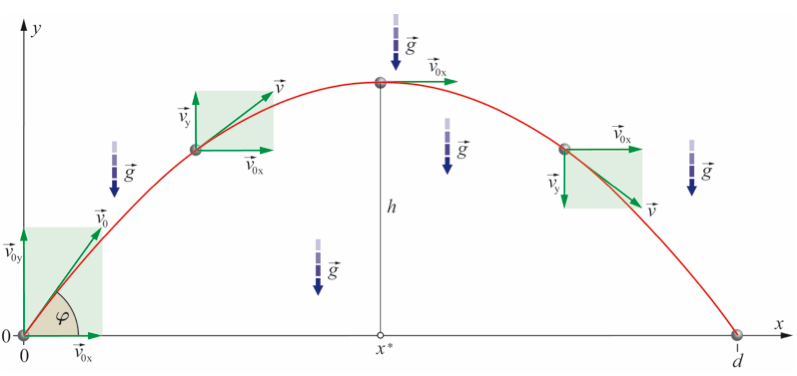
\includegraphics[width=0.9\linewidth]{images/schiefer_wurf}
\end{minipage}
\hfill
\begin{minipage}[h!]{0.4\linewidth}
Bahngleichung des Schiefen Wurfs: 
\begin{align*}
y = x \cdot tan(\varphi) - \frac{g x^2}{2 v_0^2 \cos^2(\varphi)}
\end{align*}
\end{minipage}

\begin{tabbing}
	\begin{tabu} to \linewidth {X l X l}
		\toprule
		Strecke in X & $s_x = v_0 t \cos(\alpha)$ &
		Strecke in Y & $s_y = v_0 t \sin(\alpha)  - \frac{gt^2}{2}$ \\
		Maximale Wurfhöhe & $y_{max} = \frac{v_0^2 \cdot \sin^2(\alpha)}{2g}$ &
		Maximale Wurfweite & $d = \frac{v_0^2 \cdot \sin(2\alpha)}{g}$ \\
	\end{tabu}
\end{tabbing}

\begin{tabbing}
	\begin{tabu} to \linewidth {l X}
		Momentan Geschwindigkeit & $v(t) = \sqrt{v_0^2 + g^2 t^2 - 2 v_0 \sin(\alpha) gt}$ \\
		Distanz bis zur maximale Höhe & $x_{ymax} = \frac{v_0^2 \sin^2(\alpha) \cos(\alpha)}{g} = \frac{d}{2}$ \\
		Y für bekanntes X & $y = \tan(\alpha) \cdot x - \frac{g}{2 \cdot v_0^2 \cos^2(\alpha)} \cdot x^2 $ \\
		Horizontale Geschwindigkeit & $v_x = v_0 \cdot cos(\alpha)$ \\
		Vertikale Geschwindigkeit & $v_y = v_0 \cdot sin(\alpha) - g t$ \\
	\end{tabu}
\end{tabbing}

\begin{tabbing}
	\begin{tabu} to \linewidth {l X l}
		Variable & Bedeutung & SI-Einheit \\
		\midrule
		$\alpha$ & Abwurfwinkel & $\text{Grad}^\circ$ \\ 
		$g$ & Fallbeschleunigung  & $\frac{m}{s^2}$  \\ 
		$v_0$ & Betrag der Anfangsgeschwindigkeit & $\frac{m}{s}$ \\ 
		$t$ & Zeit & $s$ \\ 
		\bottomrule
	\end{tabu}
\end{tabbing}


\vfill\null
\columnbreak

\paragraph{Senkrechter Wurf und Horizontaler Wurf} \hfill \\

\begin{itemize}
	\item Beim senkrechten Wurf gelten die Formeln des Schiefen Wurfs mit dem Winkel $\varphi = 90^\circ$
	\item Beim horizontale Wurf gelten die Formeln des Schiefen Wurfs mit dem Winkel $\varphi = 0^\circ$
\end{itemize}

\begin{minipage}[h!]{0.5\linewidth}
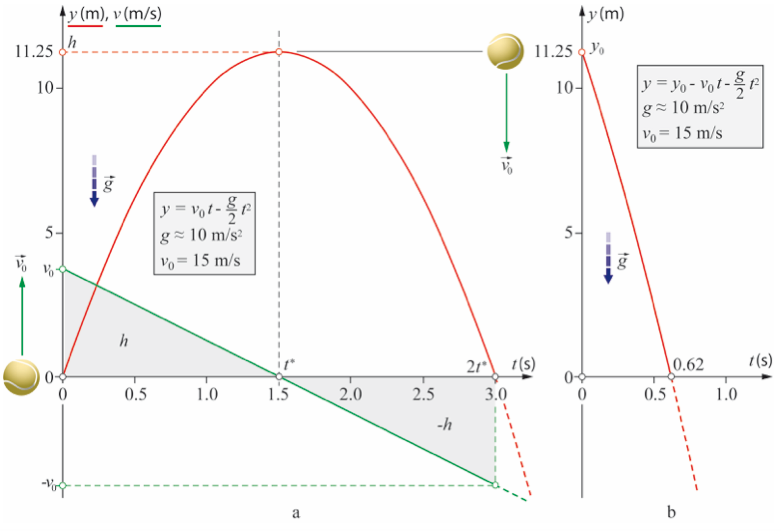
\includegraphics[width=0.9\linewidth]{images/senkrechter_wurf}
\end{minipage}
\hfill
\begin{minipage}[hbt]{0.5\linewidth}
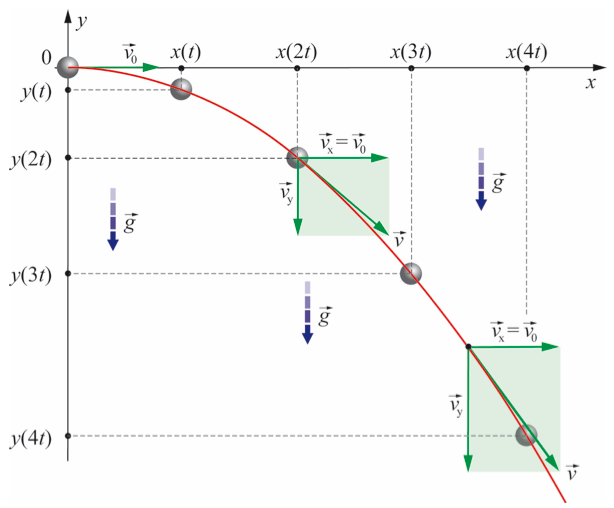
\includegraphics[width=0.9\linewidth]{images/horizontaler_wurf}
\end{minipage}

